\section{Theoretical Analysis}
\label{sec:analysis}

In this section, a theoretical analysis of the previously shown circuit was conducted. 
An audio amplifier is always divided into two separate stages, as said before. The first stage has the main function of increasing the amplitude of the voltage signal so that it can be used in the second stage. The high impedance helps to prevent signal corruption even in the first stage. Moreover, this high impedance at the output is a problem because it becomes difficult to connect the speaker without degradation of the output signal. The second stage, on the other hand, will have a low impedance so that it allows you to connect the speakers without the least possible loss of information or degradation of the signal. \par
The human ear perceives frequencies in a range of frequencies between 20 Hz to 20 kHz so we should choose coupling capacitors that behave like short circuits for these frequencies, as the coupling capacitors affect the lower cutoff frequency and thus the bandwidth.

\subsection{Step 1: DC and AC analysis for the Gain Stage}

The Gain Stage under analysis is the following:

\begin{figure}[h] \centering
\includegraphics[height=6cm]{Circuit_Gain.pdf}
\caption{Gain Stage circuit.}
\label{fig:GAIN_CIR}
\end{figure}

The capacitor bypass has the main function of preventing a loss of gain in the resistors and the main function of the resistors is to make the temperature effect stable. In the AC circuit the gain is more important and in the DC circuit the temperature effect is more important. In addition, the capacitors work as open circuits at low frequency and the current also stabilizes in the resistors thanks to the effect of temperature. At high frequencies we have the capacitors in equivalent short circuit and a bypass is used in the resistors to avoid loss of gain. \par
The values for the DC analysis, from where we garantee that the first BJT is on the FAR region, are in table~\ref{tab:TEO_DC}, and the AC results are distribuited in the input and output impedance from the gain stage (1) (table~\ref{tab:TEO_IMP}) and the gain from this stage (table~\ref{tab:TEO_GAIN}).
Both of the previous analysis were done by using the Octave script given, and as such are covered in the lectures 16 and 17.

\subsection{Step 2: DC and AC analysis for the Output Stage}

The Output Stage under analysis is the following:

\begin{figure}[h] \centering
\includegraphics[height=6cm]{Circuit_Out.pdf}
\caption{Gain Stage circuit.}
\label{fig:OUT_CIR}
\end{figure}

The values for the DC analysis, from where we garantee that the first BJT is on the FAR region, are in table~\ref{tab:TEO_DC}, and the AC results are distribuited in the input and output impedance from the gain stage (1) (table~\ref{tab:TEO_IMP}) and the gain from this stage (table~\ref{tab:TEO_GAIN}).
Both of the previous analysis were done by using the Octave script given, and as such are covered in the lectures 16 and 17.

\subsection{Step 3: AC analysis for the Audio Amplifier}

To make a more correct analysis, we have chosen to calculate the various variables using the full circuit. The DC analysis is the same as before, therefore we did not repeat it; the AC analysis was done using the following circuit:

\begin{figure}[h] \centering
\includegraphics[height=6cm]{Circuit_AC.pdf}
\caption{Audio Amplifier AC circuit.}
\label{fig:FULL_CIR}
\end{figure}

The important results from all this analysis are in the next tables:

\begin{table}[h]
  \centering
  \begin{tabular}{|l|r|}
    \hline    
    {\bf Name} & {\bf Value} \\ \hline
    \input{../mat/MAT_DC_tab}
  \end{tabular}
  \caption{The variables are of type {\it voltage} and expressed in Volt.}
  \label{tab:TEO_DC}
\end{table}

Here we can assure that the BJT's are in the FAR region, since both diferences in voltages are positive, hence ensuring the wanted behaviour.

\begin{table}[h]
  \centering
  \begin{tabular}{|l|r|}
    \hline    
    {\bf Name} & {\bf Value} \\ \hline
    \input{../mat/MAT_IMP_tab}
  \end{tabular}
  \caption{The variables of type {\it impedance} and expressed in Ohm.}
  \label{tab:TEO_IMP}
\end{table}

From this table we can see that the imput impedance of audio amplifier is almost the same as the gain stage and that the output impedance of the amplifier differs significantly from the output stage of the output stage. We can also see that the racio between the input impedance of the output stage and output impedance of the gain stage is big, allowing us to connect the two together. We can also observe that the output impedance of the gain stage is far larger than that of the output stage; this is the primary reason we use the output stage. We only print the real part of the input and output impedances in order to be coerent with the previous results.

\begin{table}[h]
  \centering
  \begin{tabular}{|l|r|}
    \hline    
    {\bf Name} & {\bf Value} \\ \hline
    \input{../mat/MAT_GAIN_tab}
  \end{tabular}
  \caption{Variables are adimentional.}
  \label{tab:TEO_RES}
\end{table}

Here we can see that the gain from the full circuit is smaller than that of both parts combined, which means that the output stage is influencing the gain stage and vice versa.

\newpage

The following figures show the plot obtained in the theoretical analysis for the gain and phase:

\begin{figure}[h] \centering
	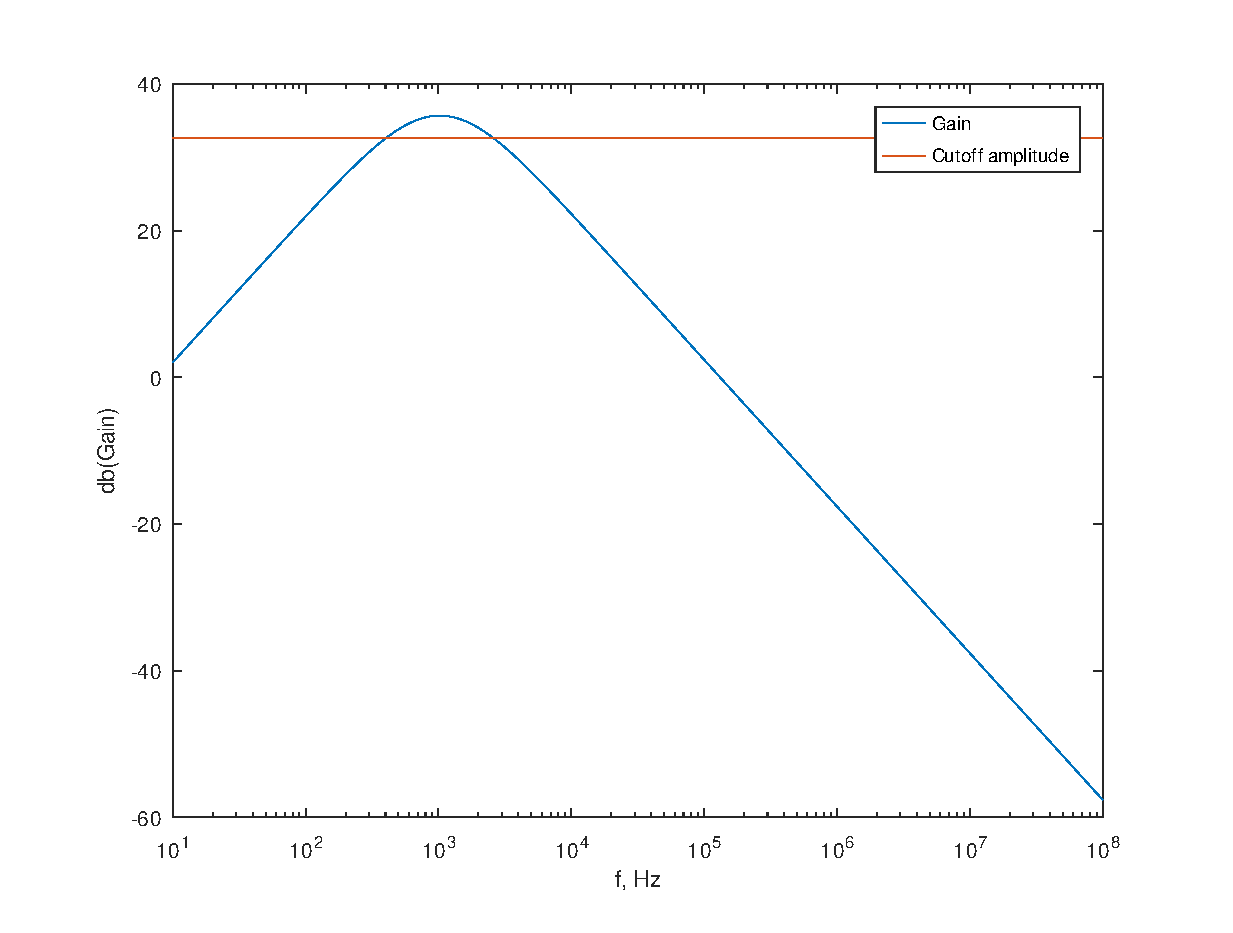
\includegraphics[height=8cm]{MAT_AB_AMP.eps}
	\caption{$db(v_{out})$ and $max(db(v_{out}))-3$.}
\end{figure}

\begin{figure}[h] \centering
	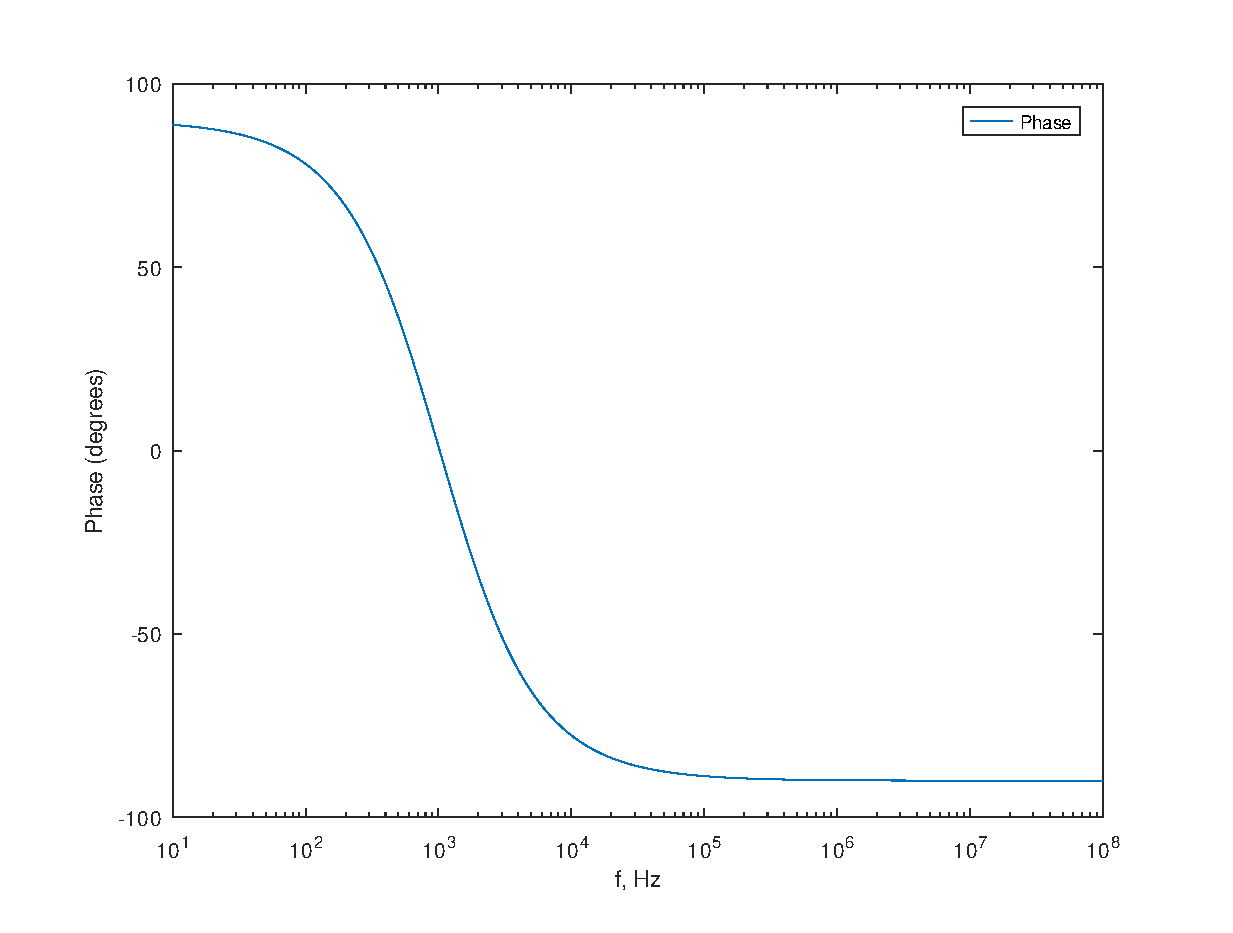
\includegraphics[height=8cm]{MAT_AB_PH.eps}
	\caption{Phasor of $v_{out}$, degrees.}
\end{figure}
